\documentclass[twoside]{projektInzynierskiMS}
\usepackage{polski}
\usepackage[utf8]{inputenc}
\usepackage{amsmath}
\usepackage{graphicx}
\usepackage{hyperref}

%\drukJednostronny

%% tytuł promotor iautor (\title to komenda standardowa)
\title{System obsługi biblioteki naukowej}
\promotor{dr inż. Zdzisław Sroczyński}


%% każdy autor musi mieć 4 argumenty: imię nazwisko, nr albumu, procent wkładu, opis wkładu
\autor{Karolina Chrząszcz}{225156}{33} 
	{Zaprojektowanie i wykonanie aplikacji serwerowej oraz mobilnej.}
	
\autor{Szymon Górnioczek}{225164}{33}
	{Zaprojektowanie i wykonanie aplikacji serwerowej oraz strony internetowej dla administratora.}

\autor{Tomasz Kryg}{225183}{33}	
	{Zaprojektowanie i wykonanie strony administratorskiej oraz mobilnej.}
	
	


%% dedykacja mile widziana
\dedykacja{To jest\\dedykacja}
%\NumeryNaPoczatku
%% numeracja wzorów tu włączona typu (1.2.3), ta druga to typu (1.2), domyślnie typu (1)
%\subsectionWzory
% \sectionWzory  

%\rozdzialy


%\literowaNumeracjaDodatkow %% włączy numerację dodatków literami
%\rzymskaNumeracjaDodatkow  %%włączy numerację dodatków liczbami rzymskimi

%% wyłączenie wyjaśnień:
\bezWyjasnien

%% standardowe komendy \newtheorem  działają jak woryginale
\newtheorem{tw}{Twierdzenie}%[subsection]
\newtheorem{twa}{Twierdzenie}%[section]
\newtheorem{dd}{Definicja}%[subsection]

\begin{document}




wstęp jest tu 


\section{Aplikacja serwerowa}
Aplikacja sewerowa LibraryApp, stanowi backend systemu bibliotecznego, oraz zapewnia narzędzia dla bibliotekarza i administratora systemu, pozwalające na zarządzanie aplikacją. Głównymi zadaniami tej aplikacji są:
\begin{itemize}
	\item zarządzanie użytkownikami i~ich uprawnienami,
	\item zarządzanie bazą danych,
	\item zarządzanie informacją na temat woluminów biblioteki wydziałowej poprzez panel administracyjny,
	\item integracja aplikacji mobilnych poprzez usługe, dającą dostep do informacji w~bazie danych.
\end{itemize}

\subsection{Użyte frameworki}

Do stworzenia aplikacji został wykorzystany \textit{Django}. Framework ten dostarcza rozwiązania takie jak:
\begin{itemize}
	\item system autoryzacji użytkowników \cite{DjangoAuth},
	\item możliwość zdefiniowania modelu danych kodem pythonowym oraz ORM wysokiego poziomu \cite{DjangoORM},
	\item automatycznie generowany i kompletny panel administracyjny \cite{DjangoAdmin},
	\item narzędzie do tworzenia serwisów webowych - \textit{Django REST framework} \cite{DjangoRest},
	\item wsparcie dla wielojęzycznych aplikacji (w tym język polski) \cite{DjangoTranslation},
\end{itemize}
które kompletnie pokrywają potrzeby aplikacji LibraryApp. Oprócz tego, jak można przeczytać na oficjalnej stronie \textit{Django} \cite{DjangoOfficial}, framework jest zaprojektowany~w taki sposób, aby robić częste zadania web-deweloperskie szybko i prosto. W praktyce oznacza to, że powstaje mało kodu aplikacji, dzięki czemu będzie on łatwiejszy do zrozumienia i modyfikowania. Obszerna i aktualna dokumentacja, dostepna na stronie projektu, oraz duża społeczność korzystająca z \textit{Django} sprawia, że rozwój aplikacji jest łatwiejszy.

\subsubsection{Modele Django}
W \textit{Django} modele danych definiuje się jako klasy Python, które dziedziczą po \verb`django.db.models.Model` \cite{DjangoModel}. Na podstawie takiej klasy \textit{Django} automatycznie generuje tabele w bazie danych, każdy atrybut modelu reprezentuje pole w tabeli. Przykładowo, z modelu zdefniowanego w ten sposób:

\begin{verbatim}
class Category(models.Model):
    category_id = models.CharField(
        max_length=200,
        unique=True,
        verbose_name='Id kategorii'
    )
    category_name = models.TextField(
        verbose_name='Nazwa kategorii'
    )
\end{verbatim}
zostanie wygenerowana tabela w bazie danych:
\begin{verbatim}
CREATE TABLE `libraryapp_category` (
	`id`	integer NOT NULL PRIMARY KEY AUTOINCREMENT,
	`category_id`	varchar(200) NOT NULL UNIQUE,
	`category_name`	text NOT NULL
);
\end{verbatim}

\subsection{Model danych}

Model danych został zaprojektowany na podstawie specyfikacji:
\begin{itemize}
	\item arkusza kalkulacyjnego z danymi (\verb`dane-prog-bibl.xlsx`),
	\item dokumentu zawierającego opis pól (\verb`BIBLIOTEKA-program.docx`).
\end{itemize}

Arkusz \verb`dane-prog-bibl.xlsx` składa się z 3 zakładek:
\begin{itemize}
	\item KSIAZKA,
	\item KATEGORIE,
	\item PRZYPISANIE\_KATEGORII.
\end{itemize}

Zakładka KSIAZKA składa się z kolumn:

\begin{itemize}
	\item SYG\_MS,
	\item SYG\_BG
	\item OZN\_OPDOW,
	\item TYTUL,
	\item TOM,
	\item ROK,
	\item ISBN/ISSN,
	\item TYP,
	\item DOSTEPNOSC.
\end{itemize}

Zakładka KATEGORIE składa się z kolumn: 
\begin{itemize}
	\item ID\_KATEGORII,
	\item KATEGORIA.
\end{itemize}
 
Zakładka PRZYPISANIE\_KATEGORII składa się z kolumn:

\begin{itemize}
	\item SYG\_MS,
	\item ID\_KATEGORII.
\end{itemize}
 

Na podstawie takiej struktury danych zostały zaprojektowane dwa modele:
\begin{itemize}
	\item \verb`Book`, odpowiadający danym z zakładek KSIAZKA i PRZYPISANIE\_KATEGORII,
	\item \verb`Category`, odpowiadający danym z zakładki KATEGORIE.
\end{itemize}

Wszystkie definicje modeli znajdują się w pliku \verb`/libproject/libraryapp/models.py`.

\subsubsection{Model Book}

Model danych \verb`Book` jest zdefiniowany jako model \textit{Django}, składa się z pól:

\begin{itemize}
	\item \verb`signature_ms`, \\
		typu: \verb`IntegerField`, \\
		odpowiada danym z kolumny: SYG\_MS,
	\item \verb`signature_bg`, \\
		typu: \verb`CharField`, \\
		odpowiada danym z kolumny: SYG\_BG,
	\item \verb`responsibility`, \\
		typu: \verb`TextField`, \\
		odpowiada danym z kolumny: OZN\_OPDOW,
	\item \verb`title` \\
		typu: \verb`CharField`, \\
		odpowiada danym z kolumny: TYTUL,
	\item \verb`volume` \\
		typu: \verb`CharField`, \\
		odpowiada danym z kolumny: TOM,
	\item \verb`year`\\
		typu: \verb`IntegerField`, \\
		odpowiada danym z kolumny: ROK,
	\item \verb`isbn_issn` \\
		typu: \verb`CharField`, \\
		odpowiada danym z kolumny: ISBN/ISSN,
	\item \verb`type` \\
		typu: \verb`CharField`, \\
		odpowiada danym z kolumny: TYP, \\
		przyjmuje wartości: \verb`'podręcznik'', \verb`'inny'`, \verb`'zbiór zadań'`,
	\item \verb`availability` \\
		typu: \verb`CharField`, \\
		odpowiada danym z kolumny DOSTEPNOSC, \\
		przyjmuje wartości: \verb`'dostępna'`, \verb`'wypożyczona'`, \verb`'czytelnia'`.
	\item \verb`categories` \\
		typu: \verb`ManyToManyField`, \\
		odpowiada danym z zakładki PRZYPISANIE\_KATEGORII.
\end{itemize}

\subsubsection{Model Category}

Model danych \verb`Category` jest zdefiniowany jako model \textit{Django}, składa się z pól:

\begin{itemize}
	\item \verb`category_id`, \\
		typu: \verb`CharField`, \\
		odpowiada danym z kolumny: ID\_KATEGORII,
	\item \verb`category_name`, \\
	typu: \verb`TextField`, \\
	odpowiada danym z kolumny: KATEGORIA.
\end{itemize}

\subsection{Ważne klasy}

Oprócz modeli opracowanych na podstawie dostarczonych danych, zostały zaprojektowane jeszcze klasy takie jak: \verb`CategoryTree`, \verb`Dictionary`, \verb`Query`. 

\subsubsection{Klasa CategoryTree}

Ze względu na wymagania opisane w punktach \textit{10 Kategoria główna} i \textit{11 kategoria szczegółowa}, dokumentu \verb`BIBLIOTEKA-program.docx`, dotyczące podziału kategorii na "kategoria główna" i "kategoria szczegółowa", została zaimplementowana klasa która przedstawia tę relację między kategoriami. Kategoria główna to taka, której id jest postaci "\verb`G_x`", gdzie \verb`x` to ciąg cyfr, na przykład \textbf{G\_00:ALGEBRA}.
 Kategoria główna może mieć kategorie szczegółowe, których id jest postaci "\verb`G_x-S_y`", gdzie \verb`x` i \verb`y` to ciągi cyfr, część znajdująca się przed "\verb`-`" to id kategori głownej. Zatem kategoria \textbf{G\_00-S\_04:algebry Boole’a}, jest kategorią szczegółową kategori \textbf{G\_00:ALGEBRA}. 
 
Klasa \verb`CategoryTree` składa się z pól:
\begin{itemize}
	\item \verb`main_category`, 
		zawiera obiekt \verb`Category`,
		odpowiadający kategorii głównej,
	\item \verb`subcategories`, 
		zawiera tablicę obiektów \verb`Category`,
		odpowiadającym kategoriom szczegółowym.
\end{itemize}
Przykład:
\begin{verbatim}
{
    "main_category": {
        "category_id": "G_22",
        "category_name": "TOPOLOGIA"
    },
    "subcategories": [{
            "category_id": "G_22-S_00",
            "category_name": "topologia ogólna"
        },
        {
            "category_id": "G_22-S_01",
            "category_name": "topologia algebraiczna"
        }
    ]
}
\end{verbatim}

\subsubsection{Klasa Dictionary}
W celu dostarczenia do aplikacji mobilnych informacji o wartościach jakie mogą przyjmować niektóre pola w bazie danych oraz ułatwić w przyszłości modyfikowanie zakresu tych wartości, została zaimplementowana klasa \verb`Dictionary`. Obiekt tej klasy zawiera składa się z pól:
\begin{itemize}
	\item \verb`types`, tablica zawierająca wartości jakie może przyjać pole \verb`Book.types`,
	\item \verb`availability_types`, tablica zawierająca wartości jakie może przyjać pole \verb`Book.availability`.
\end{itemize}


\begin{verbatim}
{
    "availability_types": [
        "dostępna",
        "wypożyczona",
        "czytelnia"
    ],
    "types": [
        "podręcznik",
        "inny",
        "zbiór zadań"
    ]
}
\end{verbatim}

\subsubsection{Klasa query}
Obiekt klasy \verb`query` definiuje kryteria, według których, serwis zwróci książki. Klasa \verb`query` składa się z pól:
\begin{itemize}
	\item \verb`filters` - Obiekt definiujący filtry pól książek. Pola obiektu \verb`filters` są opcjonalne. Aby otrzymać książki których tytuł jest równy pewnej wartości, obiekt \verb`filters` należy zdefiniować w następujący sposób:
	
	\begin{verbatim}
	"filters":{
	    "title":"wartość"
	}
	\end{verbatim}
	
Aby otrzymać z serwisu książki, których tytuł zawiera jakiś literał, obiekt \verb`filters` należy zdefiniować w następujący sposób:
	\begin{verbatim}
	"filters":{
	    "title__contains":"wartość"
	}
	\end{verbatim}
	
Filtry pozostałych pól definiujemy analogicznie. Filtrowanie po wielu polach zdefiniowane jest w następujący sposób:

	\begin{verbatim}
	"filters":{
	    "title__contains":"wartość",
	    "responsibility__contains": "GŁ",
	    "year":2003
	}
	\end{verbatim}
	
\item \verb`categories` - tablica id kategorii, zwrócone książki zawierają jedną z kategorii podanych w tablicy. Przykład:

	\begin{verbatim}
	"categories":["G_00","G_01-S23"]
	\end{verbatim}

Aby otrzymać z serwisu książki, które posiadają konkretny zestaw kategorii, należy zdefiniować obiekt \verb`filter`:
 
	\begin{verbatim}
	"filters":{
	    "categories":["G_00","G_01-S23"]
	}
	\end{verbatim}

\item \verb`pagination` - klasa pozwalająca na zdefiniowanie otrzymanego wycinka danych, zapobiega to zwróceniu zbyt dużej liczby danych jednoczesnie. Obiekt zawieta pola \verb`offset` - definiuje ile pierwszych pozycji odrzucić, \verb`limit` - definiuje ile pozycji może zostać zwróconych maksymalnie, podczas jednego zapytania.

\end{itemize}

Przykładowy obiekt \verb`query`:

\begin{verbatim}
"query":{
    "filters": {
        "responsibility__contains": "GŁ",
        "availability":"dostępna"
    },
    "categories":["G_00"],
    "pagination": {
        "offset":20,
        "limit":10
    }
}
\end{verbatim}

\subsection{Usługi}
Aplikacja serwerowa zapewnia usługi dające dostęp do informacji zawartych w~bazie danych. Usługi dostępne są za pomocą REST Api na środowisku uczelnianym pod adresem \verb`157.158.16.217:8000`. Do korzystania z usług nie jest wymagana autoryzacja.

\subsubsection{Usługa dostarczająca książki}
Usługa ta zwraca listę książek (\verb`book`), według kryterium zdefiniowanego przez obiekt \verb`query`.

Zapytanie:
\begin{itemize}
	\item Enpoint: /books,
	\item Method: POST,
	\item Headers: "Content-Type":"application/json",
	\item Body: JSON (application/json): \verb`query`,
\end{itemize}

Odpowiedź:
\begin{itemize}
	\item Tablica obiektów \verb`Book`.
\end{itemize}

Przykład odpowiedzi:
\begin{verbatim}
[{
    "signature_ms": 601,
    "signature_bg": "",
    "responsibility": "JAGŁOM I.M.; BOŁTIANSKI W.G.",
    "title": "Figury wypukłe",
    "volume": "",
    "year": 1955,
    "isbn_issn": "",
    "type": "inny",
    "availability": "dostępna",
    "categories": [{
        "category_id": "G_05-S_03",
        "category_name": "geometryczne pojęcie wypukłości"
    }]
}]
\end{verbatim}

\subsubsection{Usługa dostarczająca kategorie}
Usługa ta zwraca listę wszystkich kategorii przedstawionych jako obiekt \verb`CategoryTree`. 

Zapytanie:
\begin{itemize}
	\item Enpoint: /categories,
	\item Method: GET,
	\item Headers: "Content-Type":"application/json",
\end{itemize}

Odpowiedź:
\begin{itemize}
	\item Tablica obiektów \verb`CategoryTree`.
\end{itemize}

Przykładowa odpowiedź:

\begin{verbatim}
[{
        "main_category": {
            "category_id": "G_00",
            "category_name": "ALGEBRA"
        },
        "subcategories": [{
            "category_id": "G_00-S_00",
            "category_name": "algebra matematyczna"
        }]
    },
    {
        "main_category": {
            "category_id": "G_01",
            "category_name": "ANALIZA"
        },
        "subcategories": [{
            "category_id": "G_01-S_00",
            "category_name": "analiza matematyczna"
        }]
    }
]
\end{verbatim}


\subsubsection{Usługa dostarczająca słownik}
Zwraca obiekt \verb`Dictionary` zawierający wszystkie typy książek oraz typy ich dostępności.

Zapytanie:
\begin{itemize}
	\item Enpoint: /dictionary,
	\item Method: GET,
	\item Headers: "Content-Type":"application/json",
\end{itemize}

Odpowiedź:
\begin{itemize}
	\item Obiekt \verb`Dictionary`.
\end{itemize}

Przykładowa odpowiedź:

\begin{verbatim}
{
    "types": [
        "podręcznik",
        "inny",
        "zbiór zadań"
    ],
    "availability_types": [
        "dostępna",
        "wypożyczona",
        "czytelnia"
    ]
}
\end{verbatim}

\subsection{Wdrażanie}
Aby uruchomić aplikację wymagany jest jedynie zainstalowany \textit{python3.6}. Aplikację można uruchomić w systemach Linux, OS X~i Windows \cite[s. 140]{djangobook}, ten rozdział jednak opisuje proces wdrażania w systemie Linux. Skrypty załączone razem z aplikacją (\verb`setup_app.sh` oraz \verb`boot_script.sh`), są skryptami bashowymi, działającymi pod systemem Linux. 

\subsubsection{Wirtualne środowisko}
Wszystkie zależności potrzebne do uruchomienia aplikacji są instalowane wewnątrz wirtualnego środowiska, dzięki czemu proces wdrażania można~w dużej części zautomatyzować. Aby móc stworzyć wirtualne środowisko należy zainstalować paczkę \textit{virtualenv} korzystająć z polecenia:
\begin{verbatim}
sudo pip3 install virtualenv
\end{verbatim}


\subsubsection{Pobranie aplikacji}

Aplikacja jest dostępna na repozytorium \href{https://github.com/szymongor/library}{github.com/szymongor/library}, aby ją pobrać można skorzystać~z \textit{git} lub pobrać paczkę~w formie \textit{zip}~i rozpakować na maszynie, zalecane jest jednak użycie \textit{gita}, ułatwi to~w przyszłości nanoszenie zmian~w aplikacji. Szczegóły dotyczące instalacji \textit{gita} dostępne są na stronie \href{https://git-scm.com/book/en/v2/Getting-Started-Installing-Git/}{git-scm.com/book/en/v2/Getting-Started-Installing-Git/}. 

Aby ściągnąć aplikację poprzez \textit{git} należy skorzystać~z komendy:

\begin{verbatim}
git clone https://github.com/szymongor/library.git
\end{verbatim}
w rezultacie, powinien się pojawić folder library w obecnej lokalizacji. Należy otworzyć folder z aplikacją używająć komendy \verb`cd library`. Katalog powinien zawierać:

\begin{itemize}
	\item \verb`boot_script.sh` - skrypt bashowy, uruchamiający aplikację,
	\item \verb`librarysite` - folder zawierający pliki aplikacji \textit{Django},
	\item \verb`properties.py` - plik zawierający konfigurację aplikacji,
	\item \verb`setup_app.sh` - skrypt bashowy, automatycznie konfiguruje środowisko,
	\item \verb`libraryapp` - folder z plikami aplikacji Django,
	\item \verb`manage.py` - skrypt \textit{Django}, do zarządzania aplikacją,
	\item \verb`requirements.txt` - lista zależności potrzebna do uruchomienia aplikacji, zostanie automatycznie załadowana przez skrypt \verb`setup_app.sh`,
	\item \verb`static` - folder z plikami statycznimi aplikacji.
\end{itemize}



\subsubsection{Konfiguracja aplikacji}

Aby skonfigurować aplikację należy edytować plik \verb`properties.py`, np używając polecenia:
\begin{verbatim}
nano properties.py
\end{verbatim}

Konfiguracja zastosowana na środowisku Politechniki Śląskiej:
\begin{verbatim}
PROJECT_PATH="/home/biblio/libproject/"
VENV="libvenv"
HOST="157.158.16.217:8000"
LOG_FILE="logs"
SECRET_KEY='f1b($dr1^t$8!#$#!a^8xmj0+#$pnaramf1r^xd(t5a%ghjai_'
ALLOWED_HOSTS=['127.0.0.1','localhost','157.158.16.217']
USER_NAME="BibliotekaMS"
PASSWORD="tajne_haslo_nalezy_zmienic"
MAIL="admin@mail.com"
\end{verbatim}

Plik konfiguracyjny składa się z pól:
\begin{itemize}
	\item \verb`PROJECT_PATH` (!) - lokalizacja folderu library z aplikacją,
	\item \verb`VENV` (*)- nazwa wirtualnego środowiska, jeśli jeszcze nie zostało utworzone, skrypt setup\_app.sh automatycznie utworzy wirtualne środowisko o takiej nazwie,
	\item \verb`HOST` (!) - adres IP oraz port na które zostanie wystawiona aplikacja,
	\item \verb`LOG_FILE` (*) - nazwa pliku z logami aplikacji,
	\item \verb`SECRET_KEY` (!)- tajny klucz, typu string, długości 50, używany przez \textit{Django} np do podpisywania plików cookies i autoryzacji,
	\item \verb`ALLOWED_HOSTS` (!)- tablica adresów hostów/domen, które moga serwować aplikację, zabezpieczenie ze strony \textit{Django} przed atakami typu Host Header Injection,
	\item \verb`USER_NAME` (*)- nazwa użytkownika panelu administracyjnego, mającego uprawnienia administratorskie~w aplikacji,
	\item \verb`PASSWORD` (!)- hasło użytkownika,
	\item \verb`MAIL` (*)- adres email użytkownika.
\end{itemize}

Pola oznaczone "!" należy edytować, pola oznaczone "*" można edytować lub pozostawić niezmienione.

\subsubsection{Uruchomienie aplikacji}
Podczas pierwszego uruchomienia aplikacji należy wywołać komendę:
\begin{verbatim}
./setup_app.sh
\end{verbatim}
z poziomu głównego folderu aplikacji (\verb`library`). Komenda ta usuchomi skrypt, który realizuje takie zadania jak:
\begin{itemize}
	\item utworzenie wirtualnego środowiska o nazwie zdefiniowanej w pliku \verb`properties.py` jako \verb`VENV`,
	\item instalacja zależności wypisanych w pliku \verb`requirements.txt` wewnątrz wirtualnego środowiska,
	\item utworzenie konta administratora aplikacji, zgodnie z danymi podanymi w~\verb`properties.py` (\verb`USER_NAME`, \verb`PASSWORD`, \verb`MAIL`),
	\item wygenerowanie bazy danych na podstawie modelu zdefiniowanego w~pliku \verb`libraryapp/models.py`.
\end{itemize}

Aby uruchomić aplikację należy wywołać:

\begin{verbatim}
./boot_scrippt.sh
\end{verbatim}

jeśli skrypt został wykonany poprawnie powinien się ukazać komunikat podobny do tego:

\begin{verbatim}
Django version 2.0, using settings 'librarysite.settings'
Starting development server at http://157.158.16.217:8000/
Quit the server with CONTROL-C.
\end{verbatim}

a po wpisaniu w przeglądarkę adresu hosta (w tym przypadku \href{http://157.158.16.217:8000/}{157.158.16.217:8000}), powinno się ukazać okno logowania do panelu administracyjnego.

W ten sposób uruchomiona aplikacja zostanie wyłączona po zamknięciu terminala. Aby uruchomić aplikację w tle jako proces niezależny od terminala można skorzystać z wirtualnej konsoli, używając polecenia:
\begin{verbatim}
screen ./boot_script.sh
\end{verbatim}
aby opuścić wirtualną konsolę należy użyć skrótu \verb`ctrl+a` a nastepnie \verb`d`. Po opuszczeniu konsoli wyświetli się komunikat:
\begin{verbatim}
[detached from identyfikator_konsoli]
\end{verbatim}

Aby włączyć ponownie wirtualną konsolę z uruchomioną aplikacją należy użyć polecenia:

\begin{verbatim}
screen -r identyfikator_konsoli
\end{verbatim}

Polecenie: 

\begin{verbatim}
screen -ls
\end{verbatim}

wyświetli wszystkie aktywne konsole.

Aby wyłączyć aplikację można przełączyć się na wirtualną konsolę z uruchomioną aplikacją i użyć skrótu: \verb`ctrl+c`.
\subsubsection{Konfiguracja Cron}

Z powodu częstych przerw w działaniu serwera, konieczne jest uruchamianie aplikacji za każdym razem gdy serwer się uruchamia. Do tego celu został wykorzystany \textit{Cron}, program do harmonogramowania zadań \cite{linuxAdmin}. Aby skonfigurować \textit{Crona}, by uruchamiał aplikację wraz z uruchomieniem serwera, należy użyc polecenia:

\begin{verbatim}
crontab -e
\end{verbatim}

i w ostatniej lini pliku dodać wpis:

\begin{verbatim}
@reboot cd /home/<lokalizacja_projektu>/library && ./boot_script.sh
\end{verbatim}

Aby przetestować wywołanie zadania, można zdefiniować zadanie wywołujące się co minutę w analogiczny sposób:

\begin{verbatim}
* * * * * cd /home/<lokalizacja_projektu>/library && ./boot_script.sh
\end{verbatim}

po minucie powinna się uruchomić aplikacja, ważne aby po teście usunąć ten wpis z \textit{Crona}. 


\section{Panel administracyjny}

Panel administracyjny dostępny jest pod adresem \href{http://157.158.16.217:8000/admin}{157.158.16.217:8000/admin}. Po wpisaniu tego adresu w przeglądarce, powinno wyświetlić się okno logowania zatytułowane "Administracja biblioteką", przedstawione na rysunku \ref{fig:adminLogin}. Dane do logowania, jeśli nie zostały wcześniej zmienione, powinny być takie jak w pliku \verb`properties.py` (\verb`USER_NAME` i \verb`PASSWORD`). 

\begin{figure}[h]
  \centering
  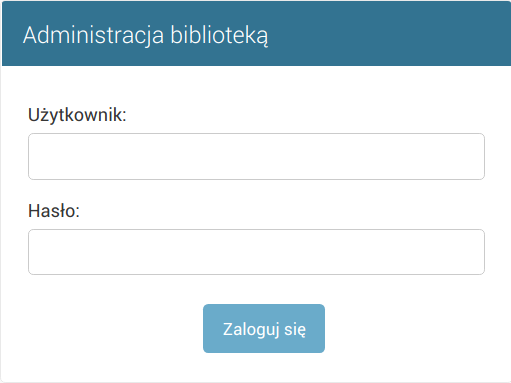
\includegraphics[width=0.4\linewidth]{img/oknLogowania.png}
  \caption{Okno logowania do panelu administracyjnego}
  \label{fig:adminLogin}
\end{figure}

Po zalogowaniu powinien się ukazać panel administracyjny do zarządzania biblioteką (rysunek \ref{fig:adminPanel}). W nagłówku strony zatytułowanym "Administracja biblioteką", znajduje się odnośnik do zmiany hasła oraz wylogowania obecnego użytkownika. Poniżej nagłówka znajdują się dwie sekcje zatytułowane "Biblioteka" i "Uwierzytelnianie i Autoryzacja". Po prawej stronie sekcja "Ostatnie działania", wyświetająca listę ostatnich zmian wprowadzonych w aplikacji.


\begin{figure}[h]
  \centering
  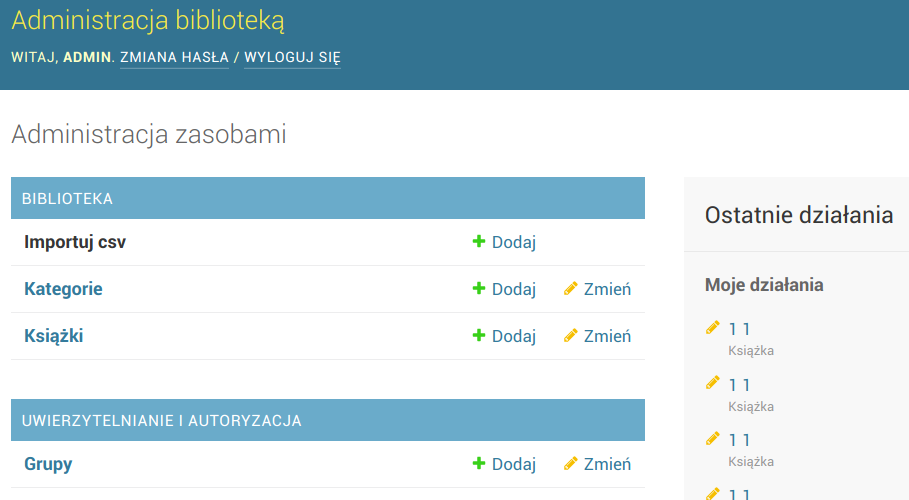
\includegraphics[width=0.4\linewidth]{img/PanelAdmin.png}
  \caption{Strona główna panelu administracyjnego}
  \label{fig:adminPanel}
\end{figure}

\subsection{Biblioteka}
W skad tej sekcji wchodzą opcje importowania plików CSV, zarządzania kategoriami i książkami.

\begin{figure}[h]
  \centering
  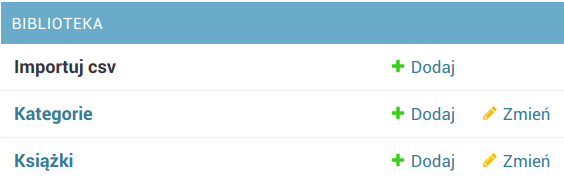
\includegraphics[width=0.6\linewidth]{img/biblioteka.png}
  \caption{Sekcja "Biblioteka"}
  \label{fig:biblioteka}
\end{figure}

\subsubsection{Importuj csv}
Po naciśnięciu "+ Dodaj", w wierszu "Importuj csv" (rysunek \ref{fig:biblioteka}), otworzy się panel zatytułowany "Dodaj CSV", widoczny na rysunku \ref{fig:importCSV}. Aby wczytać plik CSV, należy wskazać jego lokalizację (klikając przycisk "Wybierz plik") a następnie kliknąć przycisk "Zapisz". Po załadowaniu danych z pliku CSV wyświetli się lista komunikatów dotycząca statusu importowanych danych. 

\begin{figure}[h]
  \centering
  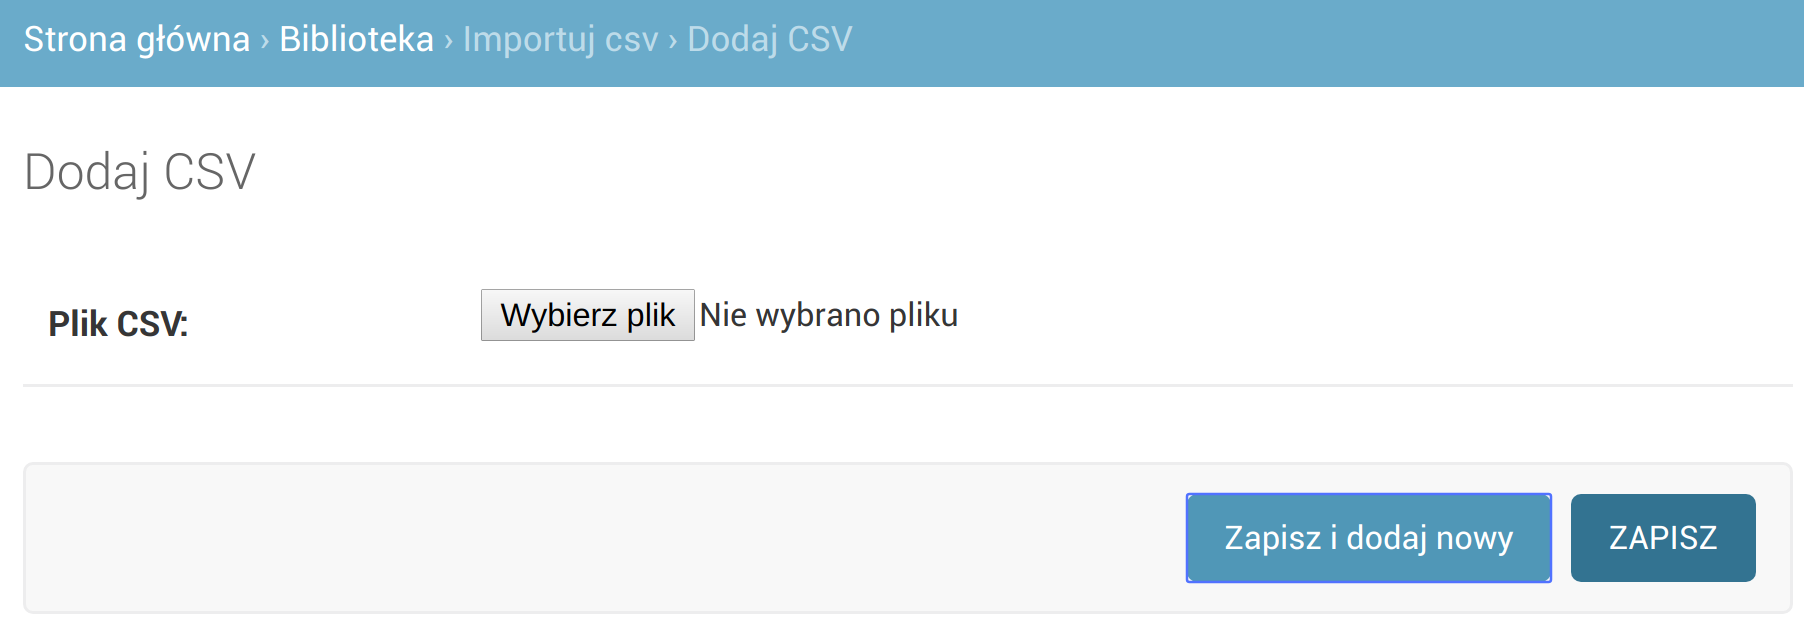
\includegraphics[width=0.6\linewidth]{img/ImportCSV.png}
  \caption{Formmularz importowania plików CSV}
  \label{fig:importCSV}
\end{figure}


Pliki CSV powinny zostać wygenerowane na podstawie arkusza kalkulacyjnego \verb`dane-prog-bibl.xlsx`, kodowanie pliku to UTF-8, symbol oddzielający pola to \textbf{,} a separator tekstu to symbol \textbf{"}. Aplikacja sama rospoznaje czy importowany plik CSV zawiera informacje z zakładki KSIAZKA, KATEGORIE czy PRZYPISANIE\_KATEGORII.

\subsubsection{Kategorie}

Wybór "Kategorie" w sekcji "Biblioteka" (rysunek \ref{fig:biblioteka}), przenosi do widoku z listą wszystkich kategorii, widocznego na rysunku \ref{fig:adminAllCategories}. Z poziomu tej listy można usuwać wybrane kategorie oraz wyszukiwać kategorie wpisując w pole tekstowe części id kategorii lub nazwy kategorii. Klikając na id kategorii w liście, otworzy się formularz edycji danej kategorii, widoczny na rysunku \ref{fig:adminEditCategory}. 

\begin{figure}[h]
  \centering
  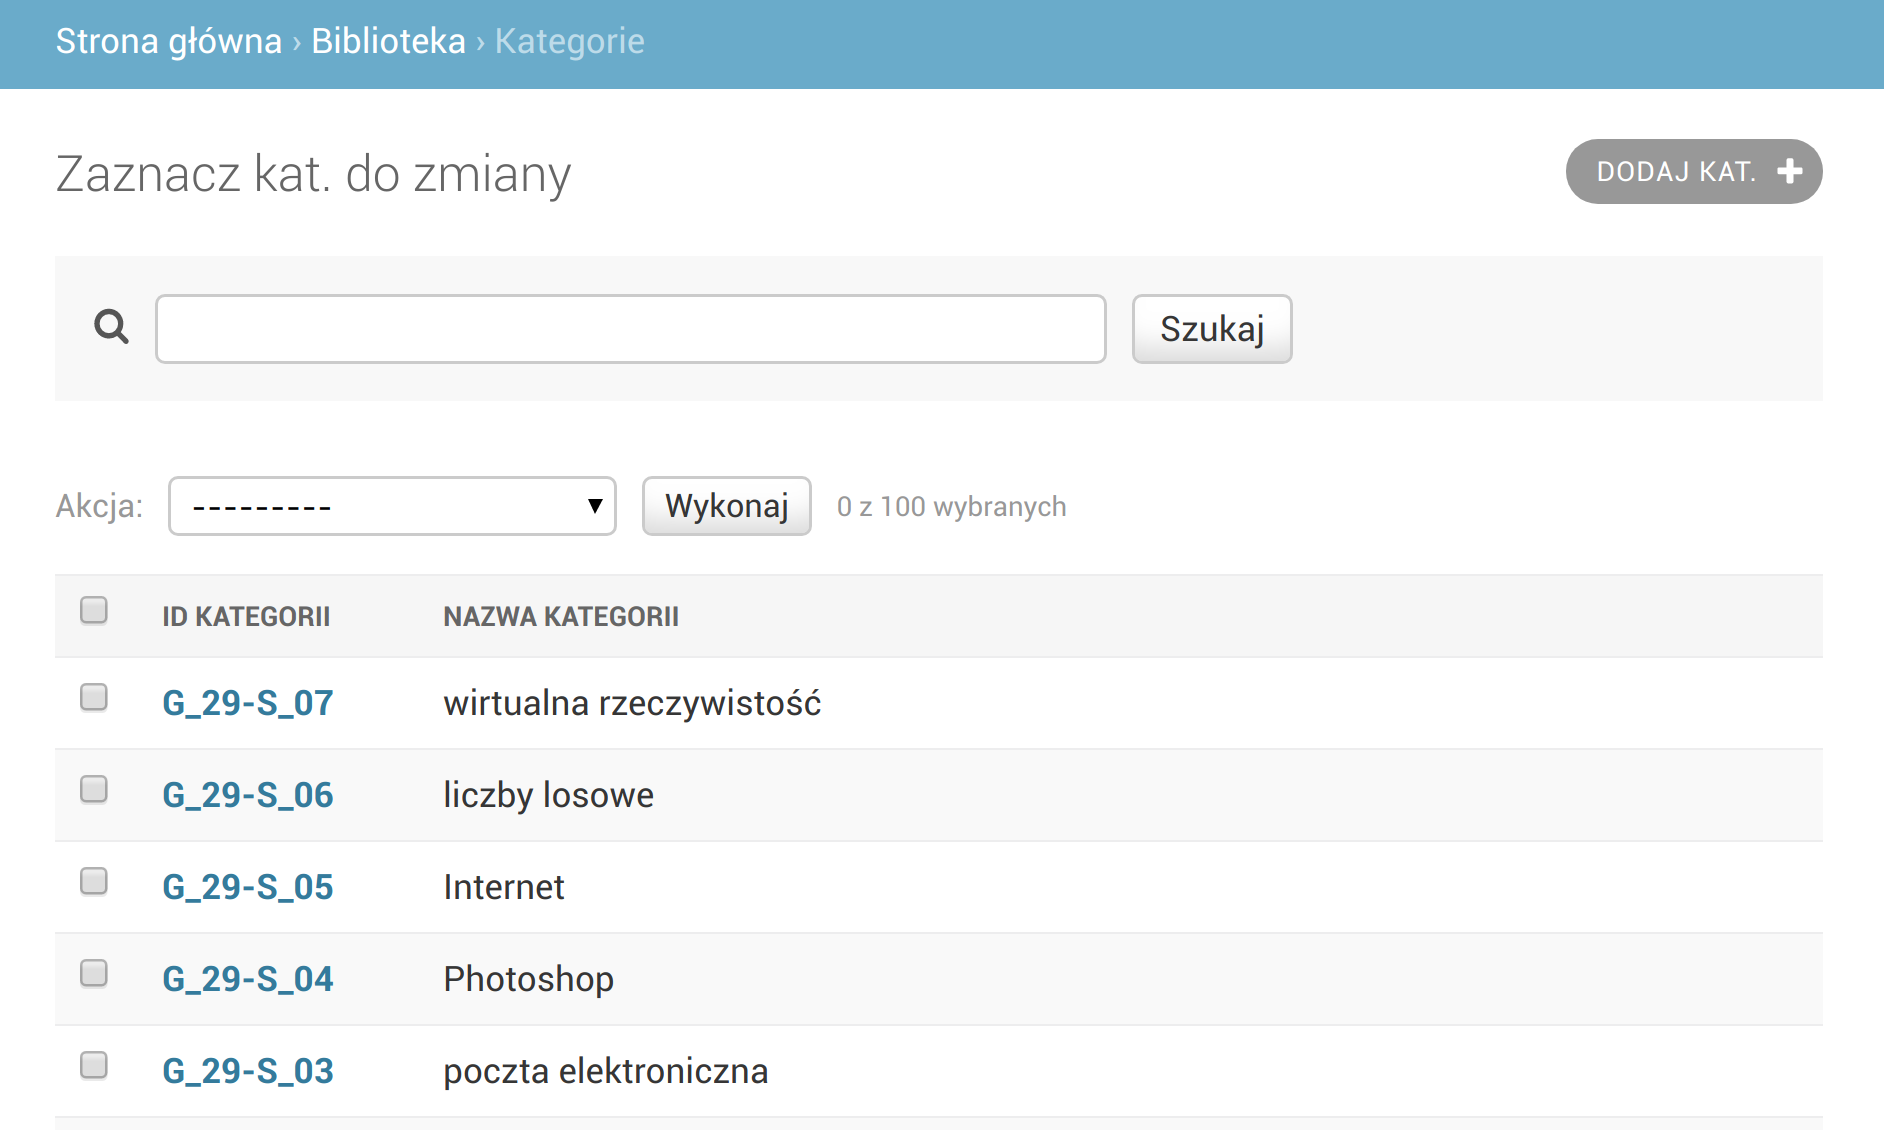
\includegraphics[width=0.4\linewidth]{img/ListaKategorii.png}
  \caption{Widok listy kategorii}
  \label{fig:adminAllCategories}
\end{figure}

Po naciśnieciu "Dodaj kat. +" (prawy górny róg na rysunku \ref{fig:adminAllCategories}), otworzy się formularz tworzenia nowej kategorii. Aby dodać kategorię główną nadajemy jej id "\verb`G_nr_kat`", gdzie "\verb`nr_kat`" to ciąg cyfr. Aby dodać kategorię szczegółową nadajemy jej id "\verb`G_nr_kat-S_nr_sub_kat`", gdzie "\verb`G_nr_kat`" to id kategorii głównej a "\verb`nr_sub_kat`" to id kategori szczegółowej.
Z poziomu okna edycji kategorii można podejrzeć historię naniesionych zmian wybierając "Historia" (prawy górny róg rysunku \ref{fig:adminEditCategory}).



\begin{figure}[h]
  \centering
  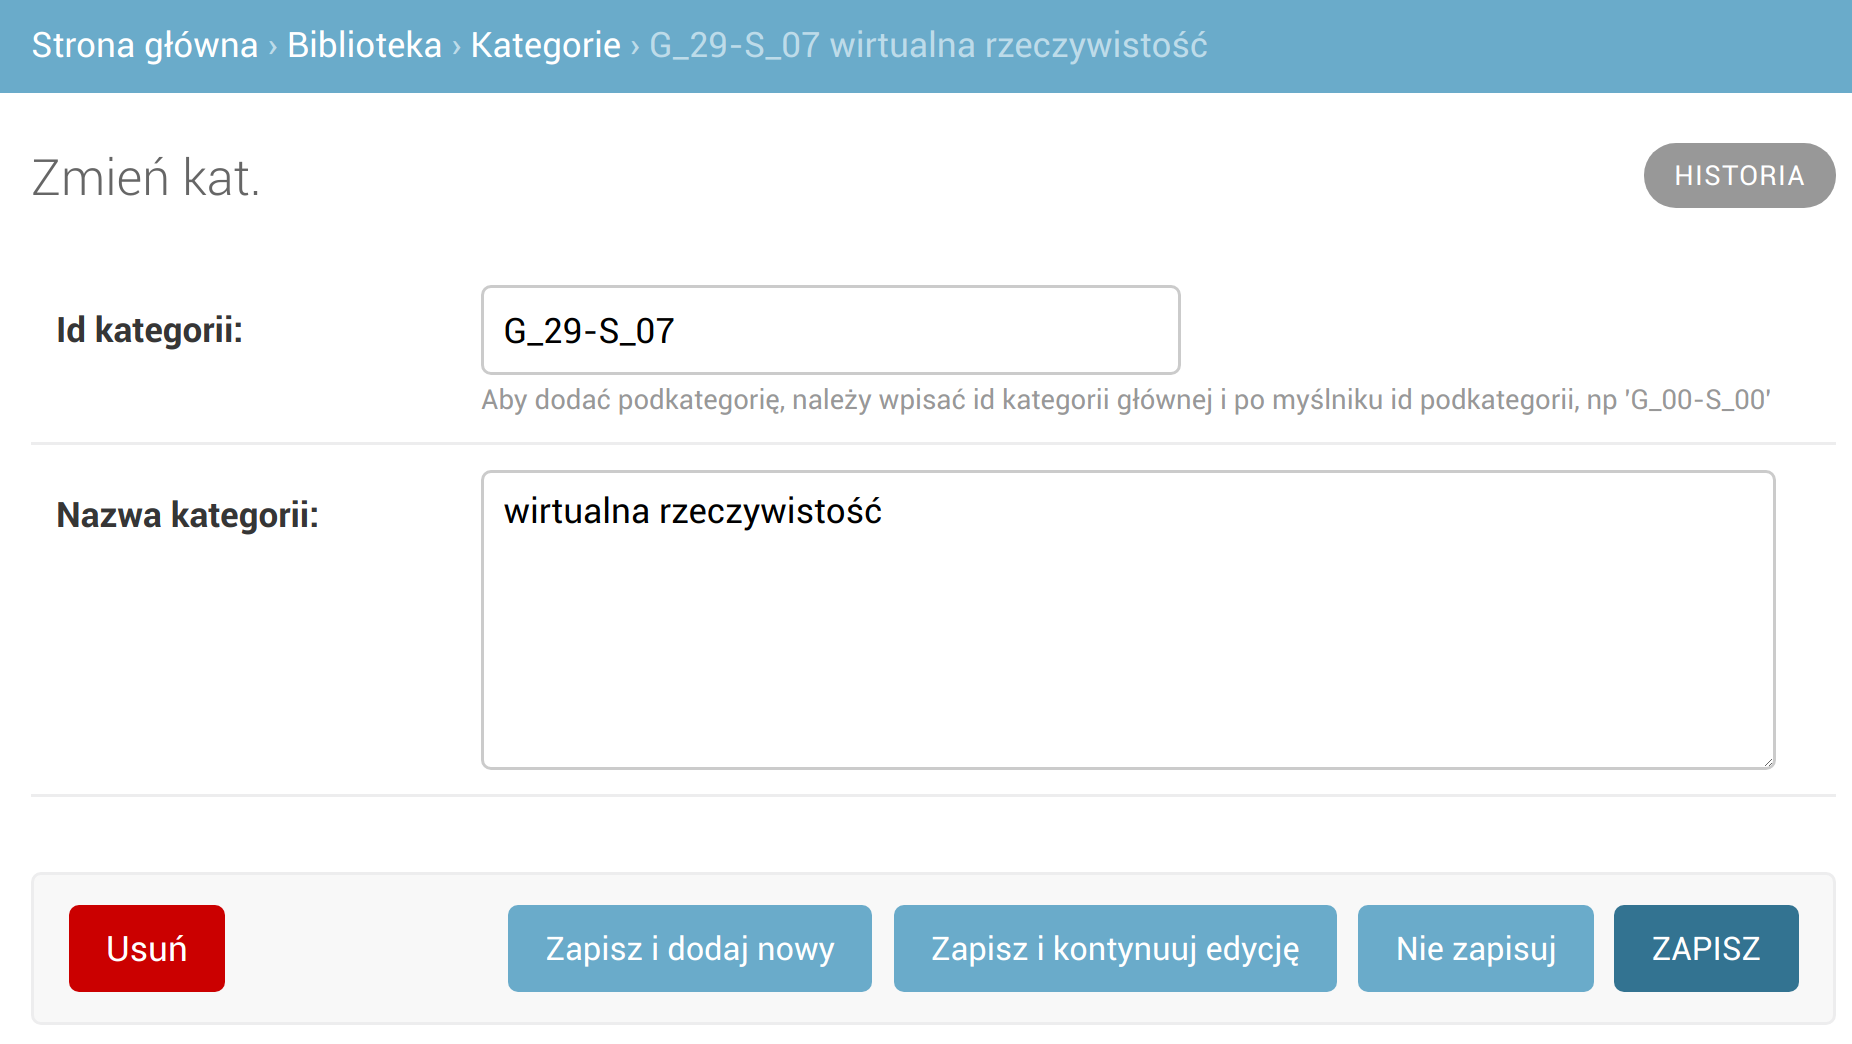
\includegraphics[width=0.4\linewidth]{img/EdycjaKategorii.png}
  \caption{Formularz edycji kategorii}
  \label{fig:adminEditCategory}
\end{figure}

\subsubsection{Książki}

Po naciśnieciu "Książki" w sekcji "Biblioteka" (rysunek \ref{fig:biblioteka}), otworzy się widok z~listą książek, widoczny na rysunku \ref{fig:adminBooks}. 

\begin{figure}[h]
  \centering
  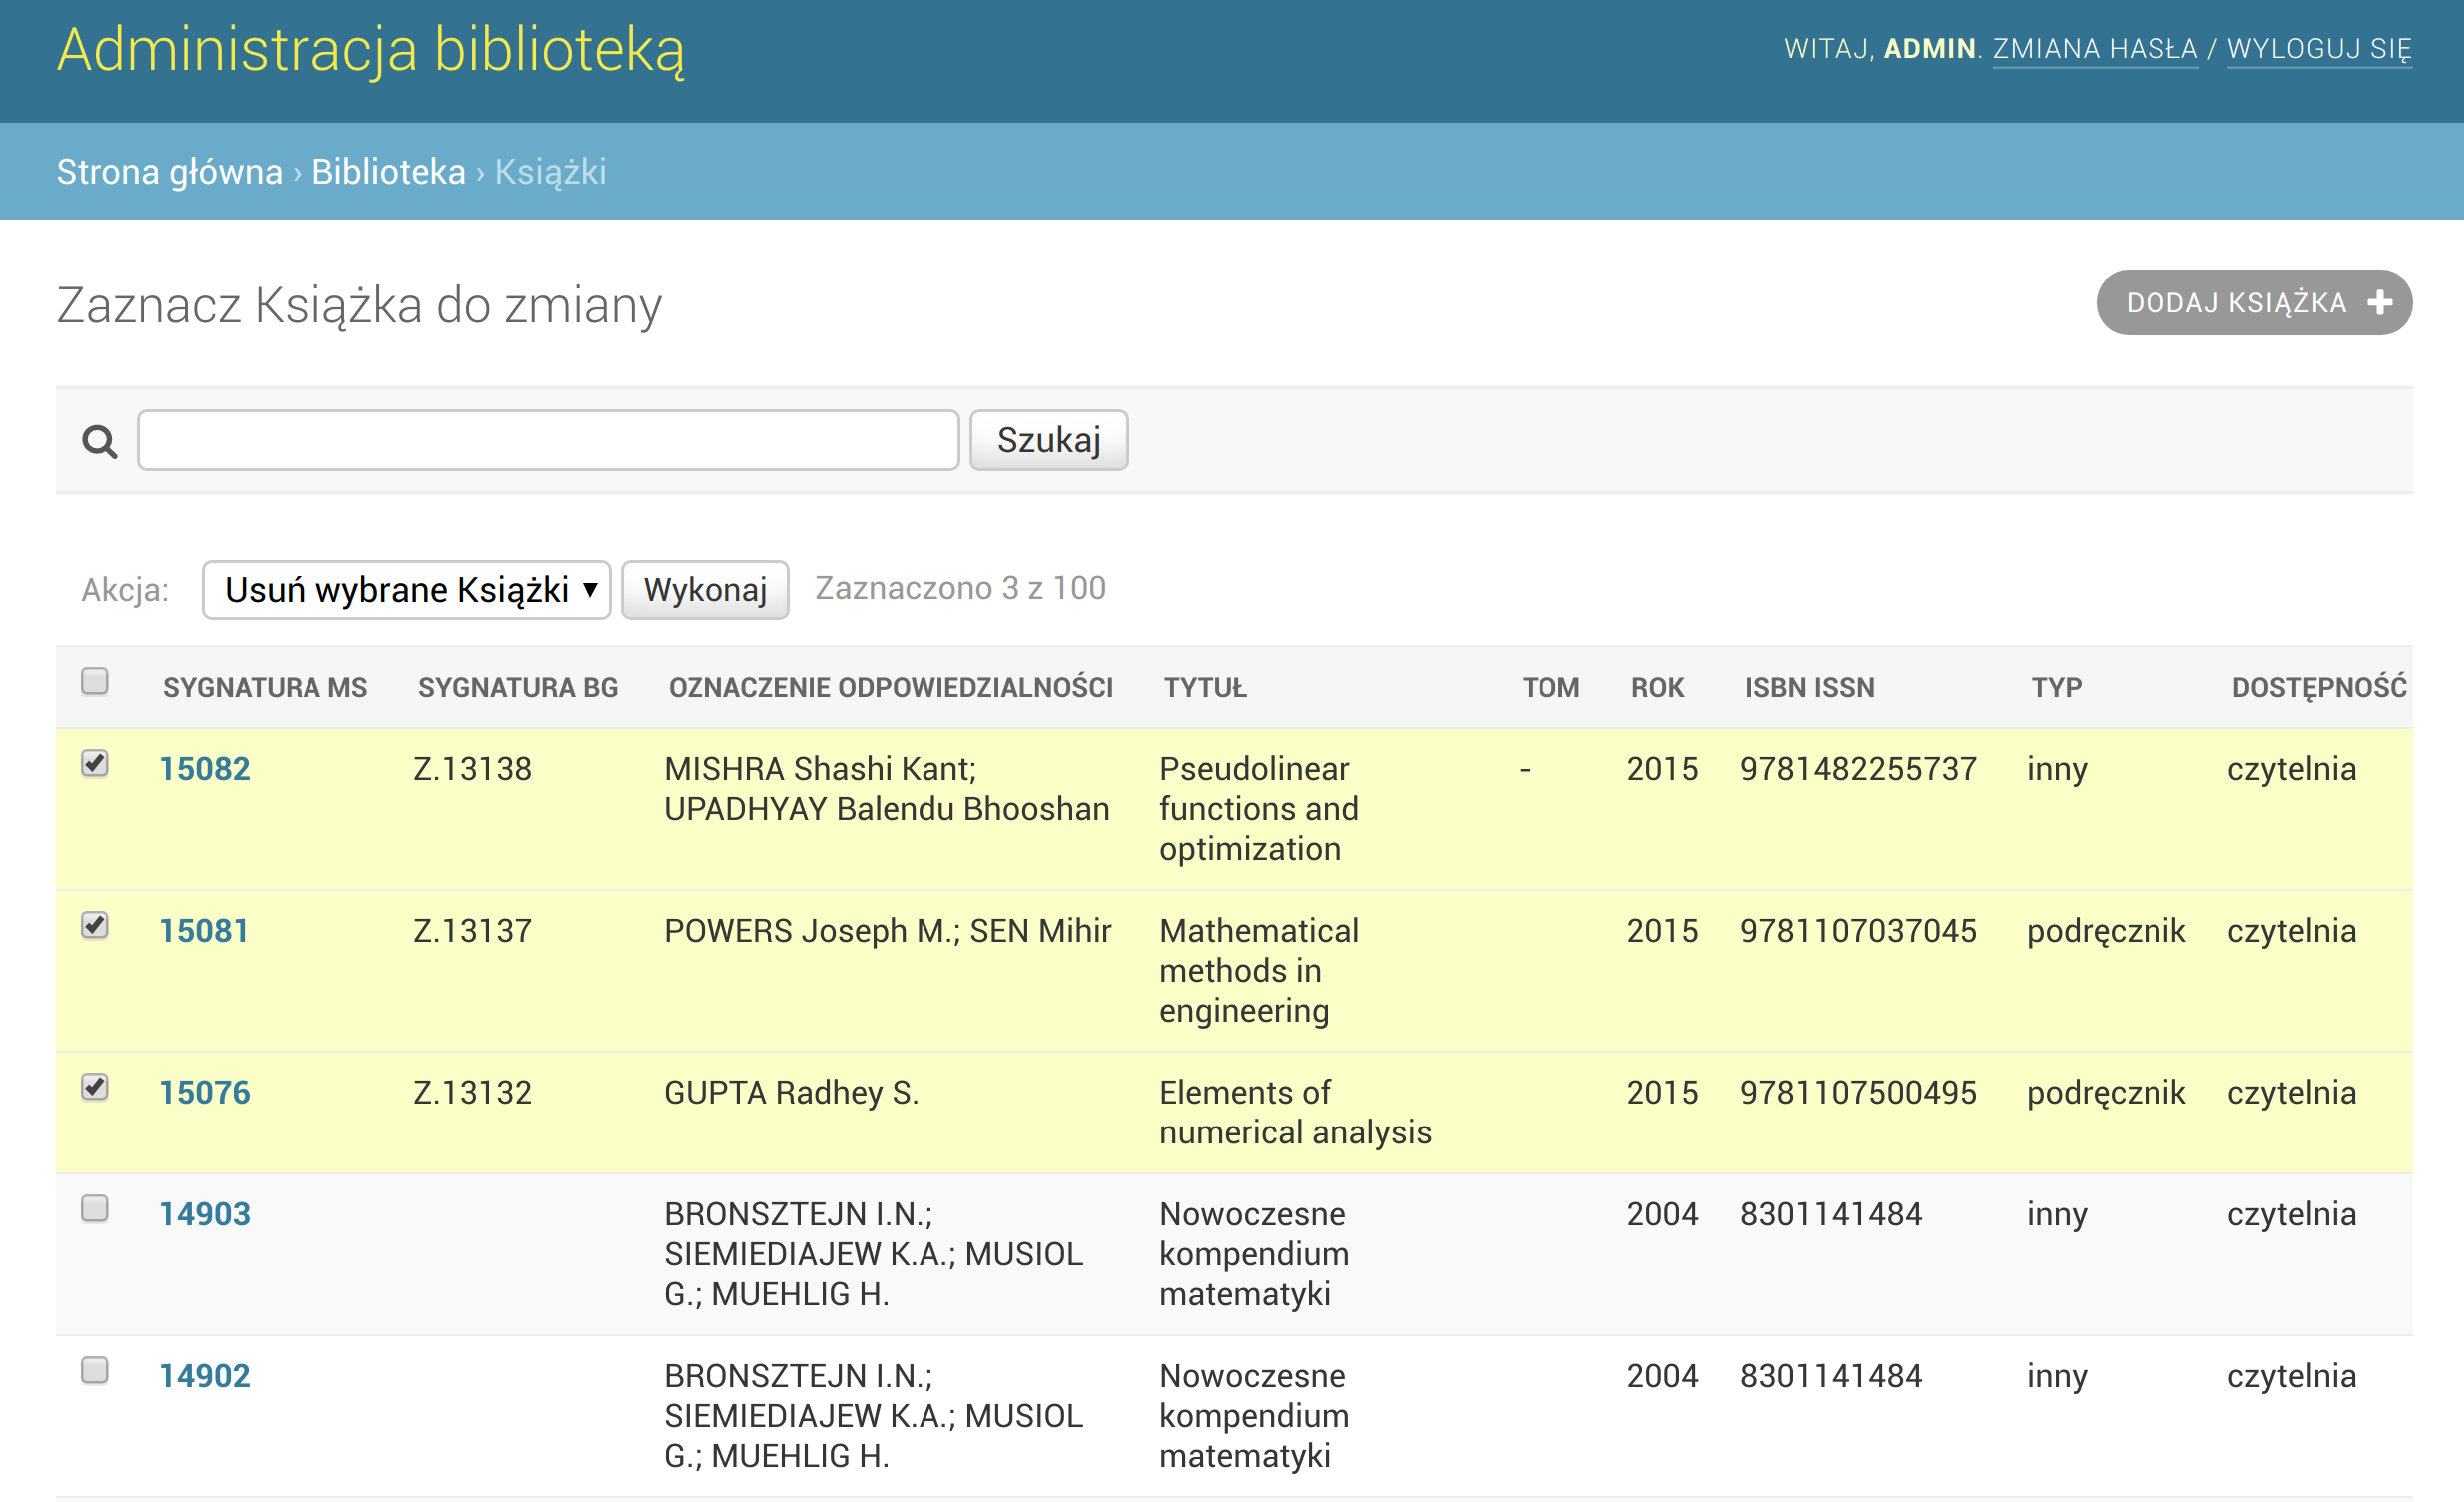
\includegraphics[width=0.4\linewidth]{img/ListaKsiazek.png}
  \caption{Widok listy książek}
  \label{fig:adminBooks}
\end{figure}

Z poziomu widoku z listą można:
\begin{itemize}
	\item wyszukiwać książek, wpisując jej id (całe) lub fragment tytułu,
	\item sortować wyświetlone książki po dowolnym zbiorze pól, klikając na nazwę tych pól w nagłówku tablicy, w odpowiedniej kolejności,
	\item usuwać wybrane książki, poprzez zaznaczenie zbioru książek i wykonanie akcji "Usuń wybrane Książki",
	\item wybrać książkę do edycji, klikając jej id na liście,
	\item dodać nową książkę, klikając "Dodaj Książka +".
\end{itemize}

Po wybraniu książki do edycji, otworzy się fromularz edycji książki widoczny na rysunku \ref{fig:adminEditBook}.

\begin{figure}[h]
  \centering
  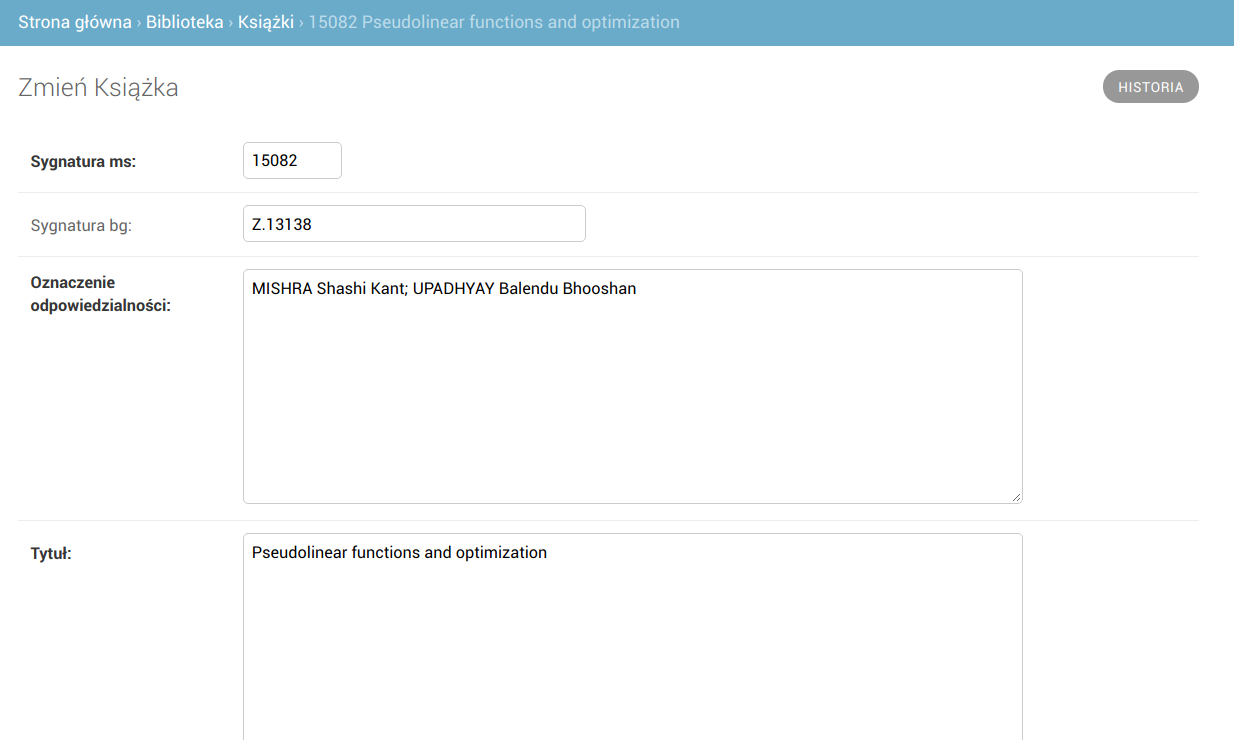
\includegraphics[width=0.4\linewidth]{img/EdycjaKsiazki.png}
  \caption{Formularz edycji książki}
  \label{fig:adminEditBook}
\end{figure}

Z poziomu okna edycji książki można przejrzeć historię naniesionych zmian wybierając "Historia". Widok zmian widoczny na rysunku \ref{fig:adminBookHistory}.

\begin{figure}[h]
  \centering
  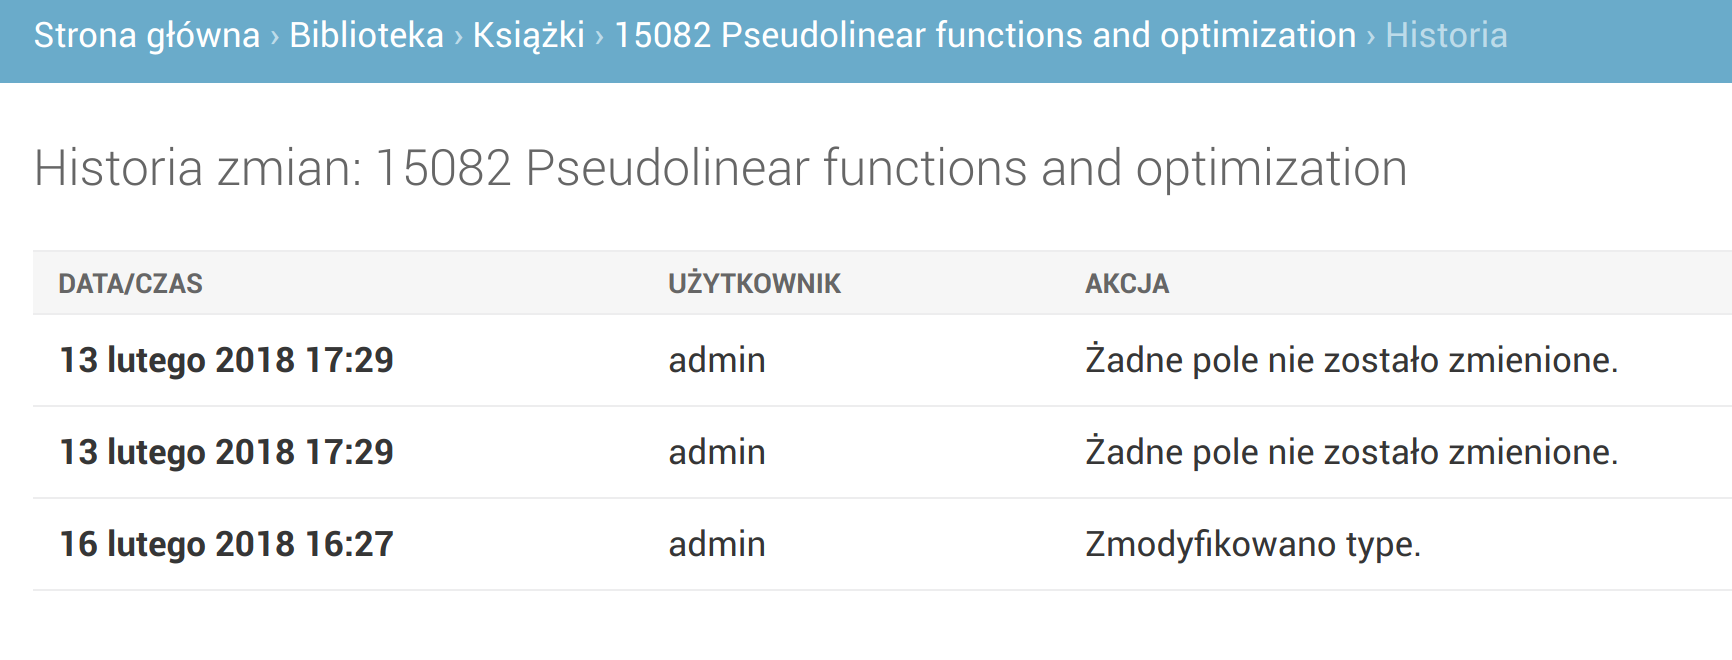
\includegraphics[width=0.6\linewidth]{img/HistoriaZmian.png}
  \caption{Widok historii zmian książki}
  \label{fig:adminBookHistory}
\end{figure}


\subsection{Uwierzytelnianie i Autoryzacja}
Sekcja ta składa się z opcji tworzenia i zarządzania kontami użytkowników i grup użytkowników.

\begin{figure}[h]
  \centering
  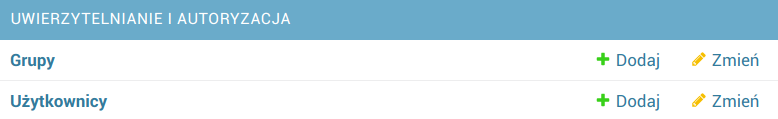
\includegraphics[width=0.6\linewidth]{img/autoryzacja.png}
  \caption{Sekcja "Uwierzytelnianie i Autoryzacja"}
  \label{fig:authSection}
\end{figure}

 Obecnie aplikacja nie wykorzystuje grup użytkowników, opcja ta została pozostawiona gdyby w przyszłości projekt miałby zawierać konta studentów z możliwością rezerwacji książek. Aby dodać nowe konto administratora biblioteki należy wybrać "+ Dodaj", w wierszu "Użytkownicy" (rysunek \ref{fig:authSection}), następnie uzupełnić formularz widoczny na rysunku \ref{fig:newUserForm} ~i zapisać.

\begin{figure}[h]
  \centering
  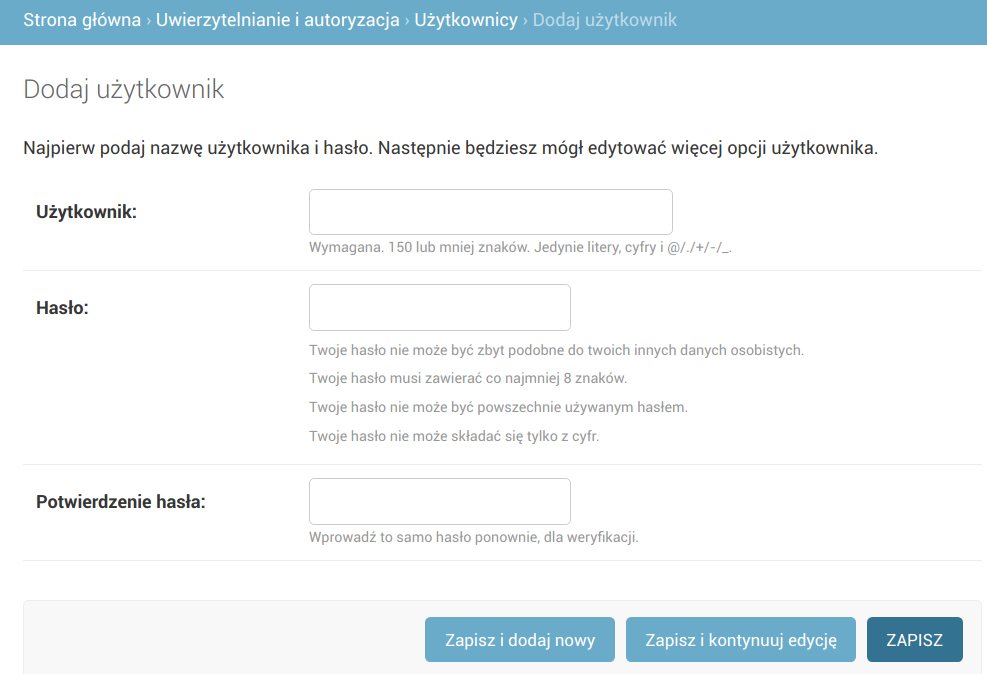
\includegraphics[width=0.6\linewidth]{img/NowyAdminForm.png}
  \caption{Formularz nowego użytkownika}
  \label{fig:newUserForm}
\end{figure}

\newpage

Nowy użytkownik powinien się teraz pojawić na liście wszystkich użytkowników aplikacji. Aby nadać mu uprawnienia administracyjne, należy wybrać na liście (widocznej na rysunku \ref{fig:usersList}) nowo dodanego użytkownika.

\begin{figure}[h]
  \centering
  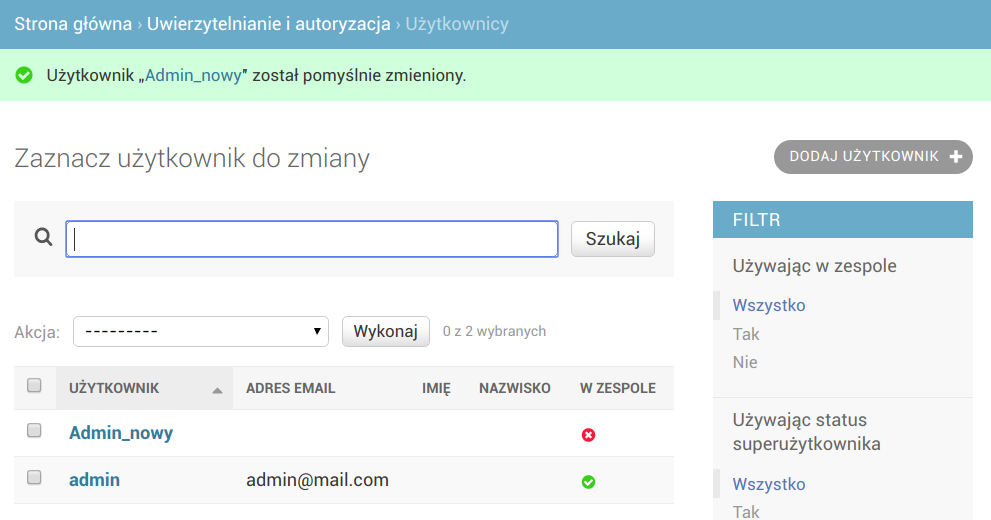
\includegraphics[width=0.6\linewidth]{img/ListaUser.png}
  \caption{Lista użytkowników aplikacji}
  \label{fig:usersList}
\end{figure}

W formularzu edycji nowego użytkownika (rysunek \ref{fig:editUser}), w sekcji "Uprawnienia", należy zaznaczyć opcję "W zespole" i zapisać.

\begin{figure}[h]
  \centering
  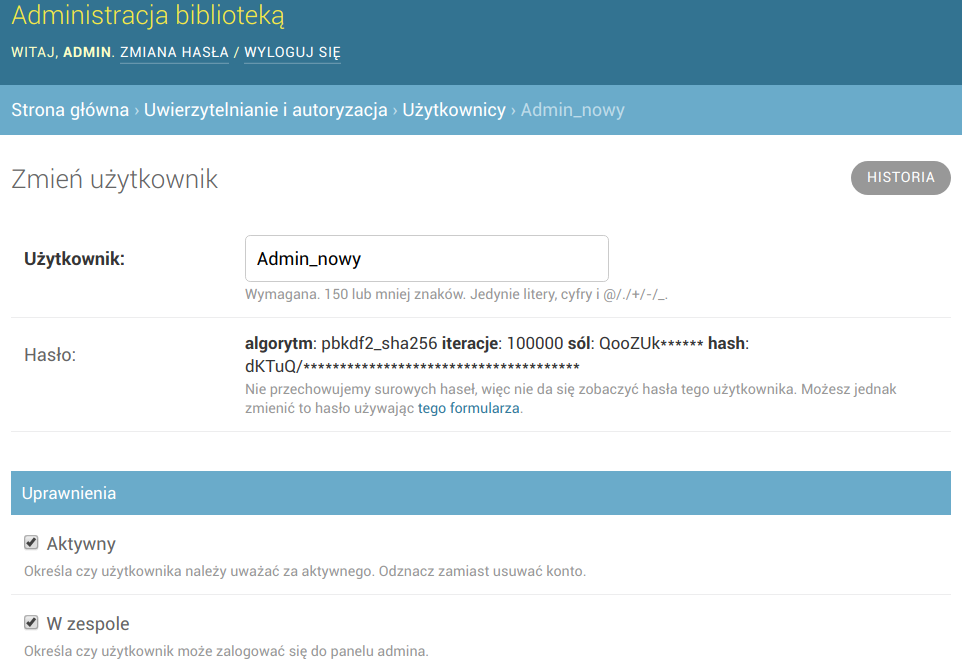
\includegraphics[width=0.6\linewidth]{img/Uprawnienia.png}
  \caption{Formularz edycji użytnownika}
  \label{fig:editUser}
\end{figure}

\begin{thebibliography}{12}
\bibitem{DjangoAuth} https://docs.djangoproject.com/en/2.0/ref/contrib/auth/ [dostęp: 10 lutego 2018]
\bibitem{DjangoORM} https://docs.djangoproject.com/en/2.0/topics/db/queries/ [dostęp: 10 lutego 2018]
\bibitem{DjangoAdmin} https://docs.djangoproject.com/en/2.0/ref/contrib/admin/ [dostęp: 10 lutego 2018]
\bibitem{DjangoRest} http://www.django-rest-framework.org/  [dostęp: 10 lutego 2018]
\bibitem{DjangoTranslation} https://docs.djangoproject.com/en/2.0/topics/i18n/translation/ [dostęp: 10 lutego 2018]
\bibitem{DjangoModel} https://docs.djangoproject.com/en/2.0/topics/db/models/ [dostęp: 10 lutego 2018]
\bibitem{DjangoOfficial} https://docs.djangoproject.com/pl/2.0/intro/overview/ [dostęp: 10 lutego 2018]
\bibitem{djangobook} A. Mele, "Django. Praktyczne tworzenie aplikacji sieciowych" Helion, 2015.

\bibitem{linuxAdmin} E. Nemeth, G. Snyder, T. Hein, B. Whaley, "Unix i Linux. Przewodnik
administratora systemów.", Wydanie IV, Helion, 2011.


\end{thebibliography}
\end{document}
